\chapter{AtariEyes package}

\label{ch:atarieyes}

This chapter describes the software realized in this thesis, that we called
``AtariEyes''. Its purpose is both to implement the ideas that have been
presented in previous chapters and to generate the experiments shown
Chapter~\ref{ch:experiments}.

Apart from being a realization of the ideas proposed, this software has some
interesting qualities:
\begin{description}
	\item [Clarity] Every method and structure has been documented.
	\item [Efficiency] Thanks to an heavy use of parallel computing libraries,
		it benefits from GPU acceleration.
	\item [User friendly] The extensive command line interface allows to
		experiment with the package as it is, or, thanks to its modular design,
		individual structures can be reused in future developments.
\end{description}

Regarding its general functionality, through the commands provided, the user
can:
\begin{itemize}
	\item Choose any \emph{environment} from the Atari~2600 collection.
	\item Train a Deep Reinforcement Learning \emph{agent}. The algorithm is
		Double DQN and the agent's model can be either the original Atari model
		(Section~\ref{sec:model-atari}) or the restricted agent
		(Section~\ref{sec:model-atari-rb}).
	\item Train the \emph{feature extractor}, because it implements every model
		and algorithm presented in Chapter~\ref{ch:fluents}.
	\item \emph{Play}, \emph{visualize} and \emph{record} any of these
		agents while they interact with the environment.
\end{itemize}

This chapter is divided in two sections: Section~\ref{sec:how-to-use}
documents how the software can be used from a user perspective;
Section~\ref{sec:implementation} is a larger part that explains some of the
most interesting details about the implementation.
%While the former is really
%useful for an high-level overview, the latter highlights some interesting
%parts which may be useful also in future developments.


\section{How to use the software}

\label{sec:how-to-use}

\subsection{Tools and setup}

The software \texttt{AtariEyes} is a Python package. It is publicly available
at the GitHub repository:
\href{https://github.com/cipollone/atarieyes}{\texttt{cipollone/atarieyes}}.
It can be installed with the \texttt{pip} commandAs any other Python package,
we just need to point to this git repository. The installation
command is:
\begin{lstlisting}[style=bash]
pip install git+https://github.com/cipollone/atarieyes
\end{lstlisting}
This installs this package from the master branch. If we need to work on some
specific revision, for example on the \texttt{develop} branch, we can append
\verb!@develop! or any other commit to the previous address.

Dependencies are automatically installed by \texttt{pip}.  In Python, it is
common to run applications inside virtual environments. Just run this
installation command within a container to avoid dependency conflicts with
other applications. One rather particular dependency is TensorFlow, which is a
famous Machine Learning library that we use for parallel computing. Following
the instructions of the specific container application, we can reuse some
preexisting system installation, if we need. Currently, the supported version
is only 2.1, but future 2.x versions might also be compatible.

The package is written in Python~3 and the minimum version required for the
interpreter is 3.7. This requirement should be met by most modern operating
systems. If that's not the case, we suggest to use \texttt{pyenv}, which
allows environment-specific Python installations.

Once installed, we can use the \texttt{atarieyes} package. As we will see, we
often use this module through its command line interface. However, if we want
just to include some structures and algorithms in other applications, we can
\lstinline[style=inlinepy]|import atarieyes|, as usual. For development it may
be also useful to look at the source code. We can clone the repository:
\begin{lstlisting}[style=bash]
git clone https://github.com/cipollone/atarieyes.git
\end{lstlisting}
This is also useful if, for any reason, some updated dependency is no longer
compatible with this package. What we can do is to \texttt{cd} to this cloned
directory, then run \texttt{poetry install}. Poetry is the container
application that we use. This command will install the exact dependency
versions that have been used during development and are guaranteed to work.


\subsection{Execution}

To run this package as a script we run the following command from the same
environment where we've installed it:
\begin{lstlisting}[style=bash]
python3 -m atarieyes
\end{lstlisting}
The reader can assume that any \texttt{atarieyes} command that we will see, is
executed by \lstinline[style=inlinesh]|python3 -m|.

\subsubsection*{Getting help}

The package provides a compete command line interface, with many options that
control the training process. In these sections we look at the most important
commands. For any doubt, we can use the \verb|--help| option, abbreviated
as \verb|-h|. When added, it prints the arguments that are supported by any
command. For example, running \lstinline[style=inlinesh]{atarieyes -h}
produces the following message\footnote{We use the
\texttt{argparse} library for parsing and generating these messages. The file
\texttt{\_\_main\_\_.py} file also acts as reference for the commands.}:
\begin{lstlisting}
usage: __main__.py [-h] [--list] [--from FROM] {agent,features} ...

Feature extraction and RL on Atari Games

positional arguments:
  {agent,features}  Choose group
    agent           Reinforcement Learning agent
    features        Features extraction

optional arguments:
  -h, --help        show this help message and exit
  --list            List all environments, then exit
  --from FROM       Load arguments from file
\end{lstlisting}

The \verb|--list| option prints the unique of every Atari game. To use any of
these games as environment, we pass its identifier to the
\verb|--env|/\texttt{-e} option, where appropriate.

The \verb|--from| option allows to execute the command and options stored some
JSON file. The JSON must be a dictionary of pairs: argument name--argument
value. The interface of this file is exactly the same of the command line
interface that we're describing. After any ``train'' command, an
\verb|args.json| is automatically saved. The purpose of this option is
allowing to repeat, resume or slightly modify a command that was previously
used.

All commands are divided in two groups. The \texttt{agent} commands regard the
RL agent, while \texttt{features} commands are related to the features
extractor.


\subsubsection*{Agents}

Three operations can be performed for the agent: \texttt{train},
\texttt{play}, and \texttt{watch}.

To train an agent we run:
\begin{lstlisting}[style=bash]
atarieyes agent train /*_ \dots _*/
\end{lstlisting}
This command has many options, some of which control the parameters of the
Double DQN algorithm. We show here just the most relevant:
\begin{description}
	\item [\texttt{-e}/\texttt{--env}] Selects the environment to use among the
		list of Atari games.
	\item [\texttt{-b}/\texttt{--batch}] Each update of the Q-Network is
		computed from a cumulative gradient of this number of samples.
	\item [\texttt{-r}/\texttt{--rate}] Chooses the learning rate associated
		to each gradient update.
	\item [\texttt{-g}/\texttt{--gamma}] Selects a discount factor.
	\item [\texttt{-c}/\texttt{--continue}] Resumes training from any
		checkpoint. Checkpoints are saved in regular intervals, according to the
		\texttt{--save} option, or when a training is interrupted with CTRL-C
		(SIGINT).
	\item [\texttt{--rb}] Trains an agent with the Restraining Bolt applied.
		When this option is absent, the agent Q-Network is that of
		Section~\ref{sec:model-atari}. When \texttt{--rb} is added, the
		restrained model from Section~\ref{sec:model-atari-rb} is used.
		The argument of this command is the IP of a running Restraining Bolt;
		often, just \texttt{localhost}.
\end{description}
There are many other options which we didn't list here.

The second command related to agents is \texttt{play}. Its purpose is to load
an agent previously trained and let it interact with the environment. This is
certainly useful to assess the performances reached. Most importantly, this
continuous play generates the stream of observations that we need in order to
train a features extractor. Some options are:
\begin{description}
	\item [\texttt{args\_file}] This mandatory argument is the path of the JSON
		file containing the exact training command of the agent.
	\item [\texttt{-c}/\texttt{--continue}] It is a mandatory argument that
		says which checkpoint to load.
	\item [\texttt{--rand-eps} {\normalfont and} \texttt{--explore-policy}]
		These two options allow to use the two custom exploration policies that
		were defined in Section~\ref{sec:exploration-policies}.
	\item [\texttt{-w}/\texttt{--watch}] To visualize the frames of the game.
		Allowed arguments are \texttt{render}, to watch the images on screen while
		the agent plays, or \texttt{stream} to send them to another running
		instance. These can be received by another instance training the
		features extractor model.
	\item [\texttt{--record}] To save a video of the agent's performance.
\end{description}


\subsubsection*{Features}

Commands that start with \texttt{atarieyes features} are related to the
features extractor. We can train the model that was developed in
Chapter~\ref{ch:fluents} and use it for prediction withing a
Restraining Bolt.

The first step is to define a set of fluents to learn, and their associated
regions. The \texttt{select} command allows to easily select the regions for
an environment. For example, to define regions in the Pong game, we run:
\begin{lstlisting}[style=bash]
	atarieyes features select -e Pong-v4
\end{lstlisting}
where \texttt{Pong-v4} is the precise name of the environment. After this
command, a frame of the game is shown. With the mouse we can do one or more
selections (press Enter to accept). The first selection is the portion of the
image where the agent should be trained (allowing to cut irrelevant parts).
Then, every following selection is a definition of a new region. After each
selection we insert at the terminal an unique name and abbreviation for that
region.

The output generated is a JSON file containing our definitions that we can now
modify and integrate. We could have written this file manually, but
\texttt{select} is a convenient way to start. The file is saved at
\texttt{definitions/}<env-name>\texttt{.json}. In our example on the Pong
environment, the output is:
\begin{lstlisting}
{
  "_frame": [ 0, 33, 160, 195 ],
  "regions": {
    "paddle_right": {
      "abbrev": "pr",
      "region": [ 131, 34, 151, 196 ],
      "fluents": []
    },
    "bottom": {
      "abbrev": "bot",
      "region": [ 0, 184, 160, 194 ],
      "fluents": []
    }
  },
  "constraints": [],
  "restraining_bolt": []
}
\end{lstlisting}
which lists each region name, abbreviation, coordinates, and fluents defined.
Now we can fill each \verb|"fluents"| with the list of symbols that we want to
define in that region.

The other two empty fields are \verb|"constraints"| and
\verb|"restraining_bolt"|. Here we write the \ldl{} formulae for the temporal
constraints (Section~\ref{sec:temporal-constraints}) and for the Restraining
Bolt temporal specification (Section~\ref{sec:rb}), respectively. The atomic
symbols of both formulae must be among the fluents we've defined above. In
this file, they are stored as lists just to improve readability. All
expressions each list are joined through conjunction in a single \ldl{}
formula. Since the \texttt{constraints} are always satisfied, we consider as
restraining specification the conjunction of both fields.

After the definitions, we're ready to train the valuation functions.
This is achieved by the \lstinline[style=bash]|atarieyes features train|, much
like we've done for the agent. Few of the many options of this command are:
\begin{description}
	\item [\texttt{--stream}] Sets the IP address of a running instance of
		\verb|agent play --watch stream| (default is \texttt{localhost}). The
		frames received are used to train this model.
	\item [\texttt{--shuffle}] Sets the size of the dataset composed by the most
		recent observations.
	\item [\texttt{-c}/\texttt{--continue}] Resumes an interrupted training from 
		a checkpoint.
	\item [\texttt{-i}/\texttt{--init}] Starts a new training but initializes
		the parameters from a checkpoint.
	\item [\texttt{--train}] The two arguments that follow are the name and the
		depth of the layer that should be trained by this command. Other parts of
		the model are not modified.
	\item [\texttt{--network}] Specifies the structure of the encoders. The
		argument of this command is a list of natural numbers. The $i$-th number
		indicates of how many hidden units is composed the $i$-th layer of each
		DBN.
\end{description}
The features extractor that we've defined in Chapter~\ref{ch:fluents} is
composed by one DBN for each region (the encoders) and the Boolean functions,
shared by all regions. The encoders, in turn, contain a stack of RBMs, which
are organized in layers. For each region, we need to train the shallow layers
first. For example as:
\begin{lstlisting}[style=bash, style=nomargin]
atarieyes features train -e Pong-v4 --network 20 3 --train bottom 0
\end{lstlisting}
Then, we proceed to the next layer just below (in this example,
\verb|bottom 1| is the next and last layer of this encoder). After each
encoder is trained, we can proceed to train the Boolean functions with
\verb|--train all -1|. Each time we proceed to a different part of the model,
we should initialize the parameters from the previous result via the
\texttt{--init} option.

Many other options, which we didn't list here, allow to personalize both
Persistent CD and the Genetic Algorithm. For example, we can tune how many
episodes are executed when computing the fitness function.

Once every part of the features extractor is trained, we can use it to make
predictions. In particular, we pass the predicted fluents values to the
Restraining Bolt. With the command \texttt{features rb} we can execute a RB
from the features extractor just trained. Some arguments are:
\begin{description}
	\item [\texttt{args\_file}] Mandatory path of the JSON file of arguments
		that generated the features extractor.
	\item [\texttt{-i}/\texttt{--init}] Model checkpoint to load.
	\item [\texttt{--stream}] IP address of the running agent to which this
		Restraining Bolt should be applied.
\end{description}


\subsubsection*{Instances}

As we can understand from the arguments of the various commands, often we need
to run more than one instance at the time. Figure~\ref{fig:cmd-instances}
shows how the instances interact in each situation.

\begin{figure}[p]
	\centering
	\subfloat[][Training a features extractor.] {
	\begin{tikzpicture}
		\node (play) [command text] {
			atarieyes agent play {\normalfont <agent-file>} --watch stream
		};
		\node (train) [command text, below=1.5cm of play] {
			atarieyes features train --env {\normalfont <env-name>}
		};
		\draw [flow] (play) -- node (mid) [midway] {} (train);
		\coordinate (frames) at ($(mid) + (1,0)$);
		\node [anchor=east, outer sep=1ex] at (mid) {$\bvec{o}_t$};
		\node [image, xshift=-0.2cm, yshift=0.2cm, opacity=0.3] at (frames)
			{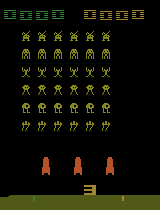
\includegraphics[width=0.8cm]{./imgs/si0.png}};
		\node [image, xshift=-0.1cm, yshift=0.1cm, opacity=0.6] at (frames)
			{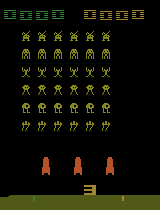
\includegraphics[width=0.8cm]{./imgs/si0.png}};
		\node [image] at (frames)
			{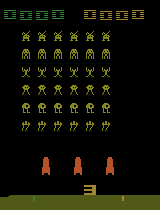
\includegraphics[width=0.8cm]{./imgs/si0.png}};
		%
		\begin{pgfonlayer}{below}
			\node [fit=(play) (train), box=orange, tight, opacity=0.5] {};
		\end{pgfonlayer}
	\end{tikzpicture}
	} \\[1.5cm]
	\subfloat[][Training a restrained agent.] {
	\begin{tikzpicture}
		\node (rb) [command text] {
			atarieyes features rb {\normalfont <features-file>} --stream
		};
		\node (train) [command text, below=1.5cm of rb] {
			atarieyes agent train --env {\normalfont <env-name>} --rb
		};
		\draw [flow] ([xshift=-2cm]train.north) --
			node (mid) [midway] {} ([xshift=-2cm]rb.south);
		\node [anchor=east, outer sep=1ex] at (mid) {$\bvec{o}_t$};
		\coordinate (frames) at ($(mid) + (1,0)$);
		\node [image, xshift=-0.2cm, yshift=0.2cm, opacity=0.3] at (frames)
			{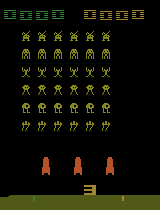
\includegraphics[width=0.8cm]{./imgs/si0.png}};
		\node [image, xshift=-0.1cm, yshift=0.1cm, opacity=0.6] at (frames)
			{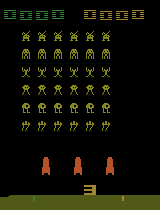
\includegraphics[width=0.8cm]{./imgs/si0.png}};
		\node [image] at (frames)
			{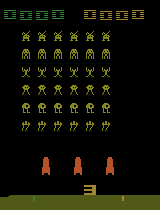
\includegraphics[width=0.8cm]{./imgs/si0.png}};
		\draw [flow] ([xshift=2cm]rb.south) --
			node [anchor=west, outer sep=1ex] {$(\vec{q}_t, r_t')$}
			([xshift=2cm]train.north);
		%
		\begin{pgfonlayer}{below}
			\node [fit=(rb) (train), box=blue!50!lightgray, tight, opacity=0.5] {};
		\end{pgfonlayer}
	\end{tikzpicture}
	} \\[1.5cm]
	\subfloat[][Training a new features extractor from a restrained agent.] {
	\begin{tikzpicture}
		\node (rb) [command text] {
			atarieyes features rb {\normalfont <features-file>} --stream
		};
		\node (play) [command text, below=1.5cm of rb] {
			atarieyes agent play {\normalfont <agent-file>} --rb --watch stream
		};
		\node (train) [command text, below=1.5cm of play] {
			atarieyes features train --env {\normalfont <env-name>}
		};
		\draw [flow] ([xshift=-2cm]play.north) --
			node (mid) [midway] {} ([xshift=-2cm]rb.south);
		\node [anchor=east, outer sep=1ex] at (mid) {$\bvec{o}_t$};
		\coordinate (frames) at ($(mid) + (1,0)$);
		\node [image, xshift=-0.2cm, yshift=0.2cm, opacity=0.3] at (frames)
			{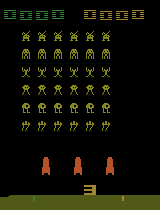
\includegraphics[width=0.8cm]{./imgs/si0.png}};
		\node [image, xshift=-0.1cm, yshift=0.1cm, opacity=0.6] at (frames)
			{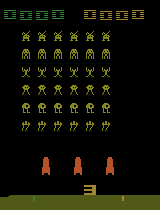
\includegraphics[width=0.8cm]{./imgs/si0.png}};
		\node [image] at (frames)
			{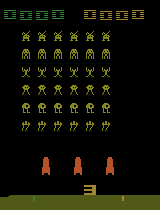
\includegraphics[width=0.8cm]{./imgs/si0.png}};
		\draw [flow] ([xshift=2cm]rb.south) --
			node [anchor=west, outer sep=1ex] {$(\vec{q}_t, r_t')$}
			([xshift=2cm]play.north);
		%
		\draw [flow] (play) -- node (mid1) [midway] {} (train);
		\coordinate (frames) at ($(mid1) + (1,0)$);
		\node [anchor=east, outer sep=1ex] at (mid1) {$\bvec{o}_t$};
		\node [image, xshift=-0.2cm, yshift=0.2cm, opacity=0.3] at (frames)
			{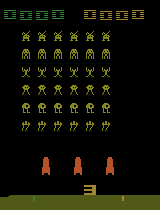
\includegraphics[width=0.8cm]{./imgs/si0.png}};
		\node [image, xshift=-0.1cm, yshift=0.1cm, opacity=0.6] at (frames)
			{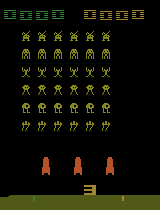
\includegraphics[width=0.8cm]{./imgs/si0.png}};
		\node [image] at (frames)
			{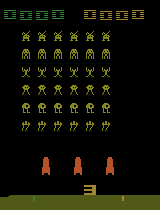
\includegraphics[width=0.8cm]{./imgs/si0.png}};
		%
		\begin{pgfonlayer}{below}
			\node [fit=(play) (train), box=orange, tight, opacity=0.5] {};
			\node [fit=(rb) (play), box=blue!50!lightgray, tight,
				opacity=0.5] {};
		\end{pgfonlayer}
	\end{tikzpicture}
	}
	\caption{How the various instances interact in each case.}
	\label{fig:cmd-instances}
\end{figure}

These instances use sockets to exchange observations, states and rewards. The
reason for this complete separation is that the main purpose of the
\texttt{atarieyes} package is to implement the Restraining Bolt and the
features extractor of Chapter~\ref{ch:fluents}, not a RL agent. In fact, there
are many modern and stable libraries implementing Deep RL agents. Thanks to
this separation, we can substitute \texttt{atarieyes agent} commands with any
software implementing a Deep RL agent. We don't need to restrict ourselves to
our implementation, not even to Double DQN. In fact, it's sufficient that the
agent's instance respects the interface of the socket messages. Since we also
provide Client--Server classes, the integration should be immediate.


\subsubsection*{Output}

To conclude this overview of the user interface, we look at the output of the 
various commands. As we've seen from \texttt{select}, the definitions for each
environment are stored in JSON files inside the \texttt{definitions/}
directory. Training commands, instead, store their result inside
\texttt{runs/}. For example,
\verb|atarieyes agent train -e Pong-v4| 
generates the following directories:
\begin{lstlisting}
runs/agent/Pong-v4/logs/0/
runs/agent/Pong-v4/models/0/
\end{lstlisting}
Every training generates ``logs'' and ``models'' directories in
unique paths composed with increasing numbers. In the example above, a new
output would be saved \verb|logs/1| and \verb|models/1|.

Inside the ``models'' directory we can find all the checkpoints saved
during training. These files can be passed as arguments to a \verb|--continue|
option, to load a saved agent. ``logs'' directory, instead, contains
\verb|args.json| and a file of TensorBoard logs. The JSON of arguments
\verb|args.json| is used for the \texttt{play} command or for the
\verb|--from| option, if we want to repeat a similar training.

The remaining files in the logs directory contain various metrics that allow
to follow the training process. These logs can be visualized with TensorBoard,
the TensorFlow visualization tool. In the example, we would run:
\begin{lstlisting}[style=bash]
poetry run tensorboard --logdir runs/agent/Pong-v4/logs/
\end{lstlisting}
For each episode, we can read: the number of steps, the cumulative reward, the
distribution of RB states, the distribution of selected actions, and other
metrics related to DQN.

The output of a \texttt{features train} command is really similar to that for
the agent: ``logs'' and ``models'' directories are saved under
\verb|runs/features| that contain the JSON of arguments, checkpoint files, and
TensorBoard logs. Intead, the main difference is the content of the log files.
Some informations that we save and can be visualized are the following:
\begin{description}
	\item [Scalar metrics] These are relevant scalar quantities that allow to
		follow the training algorithm. For RBM training, we store: free energy,
		reconstruction error, sparsity and normalization loss, learning rate.
		Instead, for the Boolean functions, we can read: average and maximum
		values of the sensitivity, consistency metrics, and fitness.
	\item [Images] Reconstructed most probable input images.
	\item [Graph] We can inspect the graph of computation of each step of the
		training algorithm. Each inner model of the features extractor has a
		different training graph. For the Boolean functions, for example, we
		observe the four steps of the genetic algorithm.
	\item [Distributions] We can observe how the model parameters are
		distributed on the real axis. This helps to investigate under/over-fitting
		and other issues. For the genetic algorithm we visualize the population
		fitness values, a projected representation of the individuals, and the
		fluents predictions.
\end{description}


\subsubsection*{\ldl{} library: \texttt{flloat}}

Temporal logic is used for two purposes: the RB restraining specification,
which indicates the agent's behaviour to reward, and the temporal constraint,
used to learn the valuation functions. They are \ldl{} formulae, written
inside each environment JSON file of definitions.

The library that we use for parsing and transforming these formulae to DFA is
called \texttt{flloat} (GitHub \href{https://github.com/whitemech/flloat}{%
\texttt{whitemech/flloat}}). The purpose of the package is to
implement the DFA transformation for two temporal logics: \ltl{} and \ldl{}.
In fact, we might alternatively use \ltl{} with minor modifications to the
source.

The initial author of this library, Favorito~\cite{bib:favorito-thesis},
started this project as a Python port of an homonymous software that was
developed in Java\footnote{GitHub
\href{https://github.com/RiccardoDeMasellis/FLLOAT}{%
\texttt{RiccardoDeMasellis/FLLOAT.}}}. Then, development has continued and,
during this thesis work, we contributed to the advancements of the
library. We helped to improve the overall stability of the software and to
write a more efficient parsing of the input languages (we use version~0.3.0).

The fields \verb|constraints| and \verb|restraining_bolt| both contain \ldl{}
expressions in a string format accepted by \texttt{flloat}.  We can refer to
this library documentation to understand what is format accepted. Since
\texttt{flloat} gets installed with \texttt{atarieyes}, we can also experiment
interactively with it.  For example:
\begin{lstlisting}[style=python]
from flloat.parser.ldlf import LDLfParser as Parser

expression = "A & [true*; A]B & <true*; ?B>tt"
formula = Parser()(expression)
automa = formula.to_automaton()
\end{lstlisting}
This is useful to check that the \texttt{expression} has the correct syntax,
and that it represents the intended temporal property (it's possible to
visualize the automaton \texttt{automa} with Graphviz). In this example,
\texttt{expression} is correctly parsed as:
\[
	A \land \lbox{\true^*; A}B \land \ldiamond{\true^*; B?} \ltt
\]



\section{Implementation}

\label{sec:implementation}

The package has a modular and comprehensible design, as we can see from the
following file structure: \\[1ex]
\hspace{2ex}
\begin{minipage}[t]{0.25\textwidth}
	\begin{forest}
		dirtree
		[atarieyes/,baseline
			[\_\_main\_\_]
			[tools]
			[streaming]
			[layers]
			[automata]
		]
	\end{forest}
\end{minipage}
\hfill
\begin{minipage}[t]{0.25\textwidth}
	\begin{forest}
		dirtree
		[atarieyes/,baseline
			[agent/
				[training]
				[playing]
				[models]
			]
		]
	\end{forest}
\end{minipage}
\hfill
\begin{minipage}[t]{0.25\textwidth}
	\begin{forest}
		dirtree
		[atarieyes/,baseline
			[features/
				[training]
				[rb]
				[models]
				[genetic]
				[temporal]
				[selector]
			]
		]
	\end{forest}
\end{minipage}
\vspace{2ex}

\noindent
Each of these files is an importable Python module (extension omitted), with a
separate functionality. We won't discuss all of them, as we only want to look
at the most interesting details of the software.


\subsection{\texttt{atarieyes} package}

There are 5 modules inside the outer scope (left column of the file hierarchy
above). \verb|__main__.py| only realizes the command line interface and
\verb|tools.py| contains generic utilities. Instead, the remaining modules are
the most interesting.


\subsubsection*{\texttt{streaming} module}

This module allows the various instances of the program to communicate. It
defines a communication protocol and the format of the messages to exchange.
The instances communicate through sockets. So, the RL agent and the
Restraining Bolt could even be on separate machines. Furthermore, this allows
our implementation of the features extractor and the Restraining Bolt to
communicate with any kind of RL agent, even implemented with some other
library. It's sufficient that the agent program does
\lstinline[style=inlinepy]|import atarieyes.streaming| to use this module
interface for exchanging messages with the Restraining Bolt.

This file defines two base classes: \texttt{Sender} and \texttt{Receiver}.
The sender is a TCP server that waits for an incoming connection from the
receiver. They only realize the basic functionality, because the specific
messages format is defined in subclasses.

\texttt{AtariFramesSender} and \texttt{AtariFramesReceiver} is a pair of
subclasses that are used to send images of the Atari games when the
\verb|--stream| option is present. Similarly, \texttt{StateRewardSender} and
\texttt{StateRewardReceiver} transmit the pair $(\vec{q}, r')$ of automaton
state and reward from the RB back to the agent.

Users can send and receive data with \texttt{send} and \texttt{receive}
methods of the respective instances in each pair.  The base classes also
provide transmit and receive buffers for an asynchronous exchange. 


\subsubsection*{\texttt{automata} module}

This module only contains one class that realizes a DFA. There are many
automata libraries available. The motivation behind this class is that we need
to be very efficient in our specific use case: running many copies of the same
automaton. In the following, let's denote with $\automa_\constraintS$ the
DFA associated to the temporal constraint.

The final layer of the features extractor model is composed by an array of
Boolean functions. As we've seen, this part is trained with a Genetic
Algorithm, which maintains a population of candidates (each individual is an
array of functions). Computing the fitness function for each individual
requires to do predictions with all of them and check the generated traces
against the temporal constraint. To do so, we continuously predict the fluents
values with each candidate, and we move each copy of $\automa_\constraintS$
accordingly. At the end of the episodes we combine the metrics to compute the
total fitness function for each candidate. Since the population can contain
thousands of candidates, it's important to have an implementation that allows
an efficient execution of thousands of parallel copies of the same DFA. 

The class \texttt{TfSymbolicAutomaton} stores the edges of the graph into a
Hash table. Each key is a pair containing the current state and the input
symbol; each value is the next state for that key. Moving through the
automaton is a simple lookup from this table. To realize both the table and
the lookup mechanism we've used the vectorial calculus of the TensorFlow
library. So, with just one call, it's possible to receive the next states for
any number of state--symbol input pairs.

The methods are:
\begin{lstlisting}[style=python]
def initial_states(self, n_instances):
	# ...

def is_final(self, states):
	# ...

def successors(self, states, symbols):

	# Lookup
	keys = self._to_keys(states, symbols)
	next_states = self.transitions.lookup(keys)
	
	return next_states
\end{lstlisting}
The automaton instance is state-less. The caller should maintain a vector of
states, created from \verb|initial_states| and transformed each time with
\texttt{successors}.

The input \texttt{symbols} is a vector of predictions, one for each candidate.
The symbols alphabet is the set of Boolean interpretations of the fluents.
This means that the space occupied by the lookup table is exponential in the
number of fluents. This is not an issue, because the \ldl{} to DFA conversion
has a double-exponential time cost, which is often a much stronger requirement
on the number of usable fluents.


\subsubsection*{\texttt{layers} module}

In Keras, TensorFlow and any modern library, Neural Networks are implemented
as a composition of layers. Although we're not required to use layers, they
allow a better organization of our models. This module defines the basic
functionality related to layers and the specific definitions of layers that
will be used in our networks.

\texttt{BaseLayer} is the base class of any layer that will be defined.
Its main role is to set some defaults and enclose the subclasses' operations
in isolated namespaces. Every layer also appears as an isolated block in the
TensorBoard graph visualization.

This module also contains an utility called \texttt{layerize}. This is a
function decorator that can be applied to functions of TensorFlow
computations. The result is a new layer class that executes the same function.
This is a very quick way of converting simple state-less computations to
layers. For example, suppose we have a simple function
\lstinline[style=inlinepy]|scale_to(inputs, in_range, out_range)| that
linearly scales the values \texttt{inputs} from the \verb|in_range| to
\verb|out_range|. Applying the decorator,
\begin{lstlisting}[style=python]
@layerize("ScaleTo")
def scale_to(inputs, in_range, out_range):
	# ...
\end{lstlisting}
defines a new class \texttt{ScaleTo}, subclass of \texttt{BaseLayer}. We can
now instantiate from this layer class:
\begin{lstlisting}[style=python]
rescaling = ScaleTo(in_range=(0, 255), out_range=(-1, 1))
\end{lstlisting}
The layer instance, \texttt{rescaling}, can be used as an atomic operation
inside other layers. Calling \lstinline[style=inlinepy]|rescaling(x)| is
equivalent to \lstinline[style=inlinepy]|scale_to(x, (0, 255), (-1, 1))|.

This module also defines:
\begin{itemize}
	\item Image preprocessing layer: scaling, cropping, resizing.
	\item Convolution block: optional padding, 2D convolution, activation
		function.
\end{itemize}

\subsection{\texttt{agent} package}

\label{sec:impl-agent}

The content of the \verb|atarieyes.agent| package is used by any
\verb|atarieyes agent| command. It contains three modules: \texttt{training},
\texttt{playing} and \texttt{models}.

The Deep RL library we've selected is called Keras-RL (GitHub
\href{https://github.com/keras-rl/keras-rl}{\texttt{keras-rl/keras-rl}})
which implements the most common algorithms using the Keras deep learning
library. The specific version used here is a slightly modified version (GitHub
\href{https://github.com/cipollone/keras-rl}{\texttt{cipollone/keras-rl}})
that uses TensorFlow~2 instead of Keras\footnote{In this version, only DQN
algorithm was completely migrated to TensorFlow. The other algorithms are not
supported.}.


\subsubsection*{\texttt{models} package}

This file contains all the necessary definitions to create a \texttt{keras-rl}
agent. Since we'll instantiate a DQN agent, the most important part is
the definition of the agent's Q-Network.

The \texttt{QAgentDef} is just an abstract class that represents a definition
of a DQN agent. Subclasses should instantiate two attributes:
\texttt{model}, which is the Q-Network of that agent, and \texttt{processor},
which allows to transform the data exchanged between the agent and the
environment.  Subclasses also define a list of metrics that allow to follow
the training process of each agent, but we mainly care about the model and
processor.

Two agents are defined in this module:
\begin{lstlisting}[style=python]
class AtariAgent(QAgentDef): # ...

class RestrainedAtariAgent(AtariAgent): # ...
\end{lstlisting}

The first of the two, \texttt{AtariAgent}, has the same structure as that of
the original DQN paper~\cite{bib:atari-deeprl}. The \texttt{model} is a
TensorFlow \texttt{Model} with the composition of layers that we've
illustrated in Section~\ref{sec:model-atari}. Essentially, it contains by a
stack of convolutional layers, followed by a final dense layer.

The \texttt{processor} is a \verb|keras-rl| structure that can transform the
observations produced by the environment, before the agent processes it. It is
used to combine a stack of the 4 most recent images into a single observation
(see the discussion on non-Markovian rewards due to moving bodies. It also
apples reward clipping and terminates episodes when the first life is lost.

The second agent, \texttt{RestrainedAtariAgent}, is used in place of
\texttt{AtariAgent} when a RB is applied (\verb|--rb| option). The
\texttt{model} of the restrained agent is a Q-Network of two inputs: the image
and the RB state. The structure of the net has been provided in
Section~\ref{sec:model-atari-rb}. The \texttt{processor} of the restrained
agent, other than performing the same operations as that of
\texttt{AtariAgent}, sends and receives data from the Restraining Bolt. Every
time the environment produces a new image, it sends this observation to the
RB and receives a new pair of state and reward in response. These inputs are
then combined with those of the environment, before passing them to the agent.

The last definitions of this modules are the three exploration policies of
Section~\ref{sec:exploration-policies}: \texttt{RepeatEpsPolicy},
\texttt{EpisodeRandomEpsPolicy} and \texttt{ExplorationPolicy}.


\subsubsection*{\texttt{training} and \texttt{playing} packages}

The \texttt{Trainer} class contained in the \texttt{training} module is
executed for any \lstinline[style=inlinepy]|agent train| command. On
initialization, it collects all the command line parameters and the
appropriate agent definition that serve to instantiate a Keras-RL agent. The
agent's class is the \texttt{DQNAgent}, which is the \texttt{keras-rl}
implementation of the (Double) DQN algorithm. Then, the method
\verb|Trainer.train| enters the main training loop.

Keras uses a very interesting concept: callbacks. A callback can be used to
insert additional computations in specific points of the training loop.  We
define two callbacks: \texttt{CheckpointsSaver}, that exports the parameters
values at regular intervals (see \verb|--save| option), and
\texttt{TensorboardLogger} which saves all the metrics to the log directories
in a format that can be visualized by TensorBoard (see \verb|--log| option).

The \texttt{playing} module follows a similar idea. It contains a
\texttt{Player} class with a \texttt{play} function. This method enters the
agent's \texttt{test} method, which is the loop of repeated play against the
environment. The callbacks defined in this module are \texttt{Streamer} to
send the images through an \texttt{AtariFramesSender}, and \texttt{Recorder}
to save a video from these frames.

The parts of the whole software regarding features are the most efficient.
We've observed that the Atari game simulator and the DQN implementation of
Keras-RL are the bottlenecks of the whole training loop. We could investigate
the use of other RL libraries in the future.


\subsection{\texttt{features} package}

This package is the largest portion of the software, because it implements all
the models and algorithms described in Chapter~\ref{ch:fluents}. The files in
this directory are used for any
``\lstinline[style=inlinesh]|atarieyes features|'' command: \texttt{training}
is used when training features, \texttt{rb} executes a Restraining Bolt from
predictions of trained features, and \texttt{selector} is the regions
selection tool (this last module doesn't need to be discussed further).
The other files define the model or participate at the training process.


\subsubsection*{\texttt{rb} module}

When we execute an ``\texttt{atarieyes rb}'' command, we start an instance
that executes a RB from trained features that continuously interacts with the
agent's instance. The class responsible for this interaction is called
\texttt{Runner}. Its only method, \texttt{run}, enters the infinite loop shown
in Listing~\ref{lst:runner-run}.
\begin{lstlisting}[style=floatpy, label=lst:runner-run,%
	caption={Infinite loop of \texttt{Runner.run} in the \texttt{rb} module.}]
while True:
		# Receive an observation
		frame, _ = self.frames_receiver.receive(wait=True)

		# Make a prediction for all fluents
		predicted = self.fluents.predict(inputs)

		# Update RB
		state, reward = self.rb.step(predicted) /*_ \label{lst:run-rb-line} _*/

		# Send RB state and reward to the agent
		self.rb_sender.send(self.states_map[state], reward)
\end{lstlisting}
The procedure is simple. At each cycle: receive an observation from the
environment (RL agent's instance), predict the fluents values from the image,
use these values to move the Restraining Bolt, send back the RB state and
reward. As we can see, this executes both the features extractor for
prediction and the RB. Of course, in order to predict the fluents values we
need to have a valuation function already trained.

The second class in this module is \texttt{RestrainingBolt} (this is the type
of the \texttt{rb} object at line~\ref{lst:run-rb-line}). The only important
detail is that it can either create a new automaton or load one previously
used. We'll see why this is important.

When the \verb|--new| option is added to an \verb|atarieyes features rb|
command, this class creates a new DFA, by combining the fields
\texttt{constraints} and \texttt{restraining\_bolt} into a single formula.
Then, it uses the \texttt{flloat} library to transform it into the
corresponding DFA. This automaton is saved in the current \texttt{logs}
directory as a file called \verb|rb.pickle|. In future runs, if both formulae
didn't change, it's important to let this class load the saved automaton.

The fist reason is efficiency, because \ldl{} to DFA is a very costly
operation. Even more important is that, if the RL agent has trained with one
automaton, it should use exactly the same automaton when testing or for
continued trainings. The reason is that the agent has learnt to associate a
state ID to a configuration of the environment. Any other permutation of the
automaton IDs would be misinterpreted by the agent.


\subsubsection*{\texttt{training} module}

Just like for the agent, a training command, in this case
\verb|atarieyes features train|, executes a \verb|Trainer.train()| method.
Its role is to instantiate a features extractor model according to the
parameters supplied (net structure, layer to train, etc), optionally
initialize the parameters from a checkpoint, and start executing the training
loop.  At each iteration it receives a new observation from the agent
instance, samples a new random batch and performs one optimization step with
the Adam optimizer.

Also in this training loop, at regular intervals, a \texttt{CheckpointsSaver}
saves the current model parameters, and a \texttt{TensorboardLogger} exports
the metrics for visualization. We care this original part more than the agent
training loop. So, the metrics are particularly detailed in this case. Also,
they only talk about quantities that are relevant for the layer currently
trained. When we train the Boolean functions, we can visualize consistency,
sensitivity and fitness; when we train a RBM we visualize the free energy and
reconstruction error, for example.

All the remaining files in this package concur for the training process or the
model definition. We'll follow a bottom up description with the few remaining.


\subsubsection*{\texttt{temporal} module}

Training the features requires to evaluate ``how much'' each candidate set of
Boolean functions satisfies the temporal constraints. For this purpose, this
module computes the ``consistency'' and ``sensitivity'' metrics from the
received traces of predicted values.

The only class is called \texttt{TemporalConstraints}. On initialization, it
converts the constraint formula to its equivalent DFA, or loads one previously
computed. It's interface is composed of just two other methods:
\texttt{observe} and \texttt{compute}. The former must be called at each time
step. As argument it receives a matrix of Boolean values, where each row is
one candidate's prediction of the fluents values. This serves to update the
relevant quantities for computing the two metrics. The latter,
\texttt{compute}, must called at the end of each episode. It has no arguments,
but returns two arrays, the value of consistency and sensitivity for each
candidate set of Boolean functions.

Both functions have been implemented with TensorFlow operations, so to
ensure a parallel computation for each candidate. The time required is weakly
dependent of the number of candidate functions.


\subsubsection*{\texttt{genetic} module}

This module contains the implementation of the Genetic Algorithm described in
Section~\ref{sec:ga-for-bools}, i.e. GA applied to Boolean functions. The file
is structured as follows. The abstract class \texttt{GeneticAlgorithm} is a
implements most of the algorithm. All the subclasses that inherit from it
just complete the algorithm with the few missing parts which are problem
dependent.

The outer interface of any \texttt{GeneticAlgorithm} is composed of two
functions. Since they are relatively simple, we report their code in
Listing~\ref{lst:ga-methods}.
\begin{lstlisting}[style=floatpy, label=lst:ga-methods,
	caption={The public interface of any \texttt{GeneticAlgorithm}.}]
def compute_train_step(self, population, fitness):

		# Compute
		population = self.reproduce((population, fitness))
		population = self.crossover(population)
		population = self.mutate(population)
		fitness = self.compute_fitness(population)

		return population, fitness

def apply(self, population, fitness):

		self.population.assign(population)
		self.fitness.assign(fitness)
		self._update_best()
\end{lstlisting}
The first, \verb|compute_train_step|, receives the current pair of population
of candidates and fitness values, and computes a new pair after one cycle of
the algorithm. We can clearly recognize the 4 basic steps: reproduction,
crossover, mutation, and fitness. \verb|apply| receives a pair of newly
computed population and fitness values and stores them into
\verb|self.population| and \verb|self.fitness|. Instead, \verb|_update_best|
saves the individual with the highest fitness value to the variable
\verb|self.best|. To execute the algorithm, the called could simply loop
over the two instructions:
\begin{lstlisting}[style=python]
population, fitness = ga.compute_train_step(ga.population, ga.fitness)
ga.apply(population, fitness)
\end{lstlisting}

The base class already defines \texttt{reproduce}, \texttt{crossover} and
\texttt{mutate}, because most operations can be executed independently of the
problem. Instead, subclasses are required to implement three functions:
\verb|initial_population|, which returns the initial population;
\verb|compute_fitness|, because is clearly problem-dependent; and
\verb|sample_symbols|, that is used when the algorithm needs to sample new
symbols (chromosomes).

For a greatest efficiency, every operation in this module has been implemented
with TensorFlow operations. In fact, reproduction, sampling, crossovers can be
implemented as parallel operations, with leads to a scalable algorithm for a
large number of individuals. This is also the reason of the separation into
\verb|compute_train_step| and \verb|apply|: keeping them separate leads to a
more efficient computation and a clearer visualization.

Every function in this class, even those defined by the subclasses, are
transformed to TensorFlow layers, thanks to \texttt{layerize}. This keeps the
model organized and simplifies the TensorBoard graph. We can see the general
structure in Figure~\ref{fig:tb-graph-ga}. The blocks we see are layers and
their content can be inspected.
\begin{figure}
	\centering
	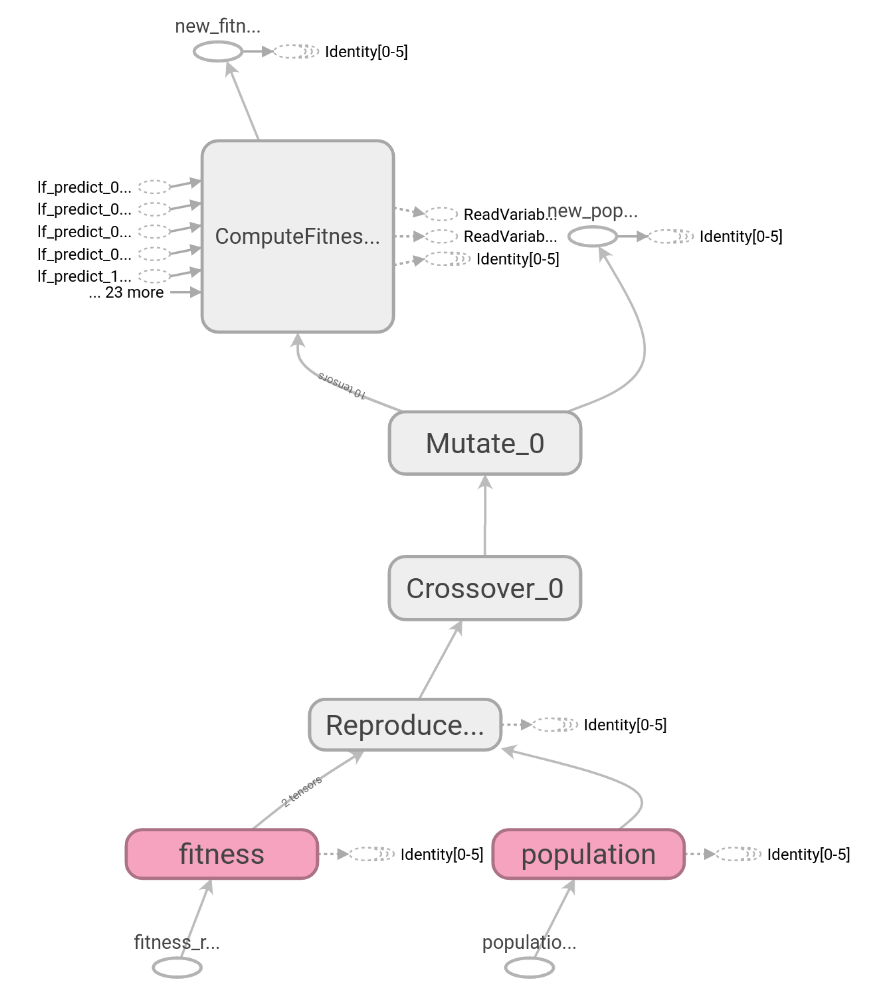
\includegraphics[height=0.45\textheight]{./imgs/ga-graph.png}
	\caption{The TensorBoard visualization of the computation graph for GA.}
	\label{fig:tb-graph-ga}
\end{figure}

We can now proceed to apply this algorithm to learning the Boolean functions,
just like we've discussed in Section~\ref{sec:ga-for-bools}.
The class \texttt{BooleanFunctionsArrayGA} is a subclass of
\texttt{GeneticAlgorithm} that defines the missing methods for the problem of
learning the Boolean functions.

This class defines, through \verb|initial_population| and
\verb|sample_symbols|, a population composed of arrays of Boolean rules,
exactly those shown in Figure~\vref{fig:boolean-rules}. Essentially, each
individual is composed by the concatenation of encoded Boolean rules. We don't
need to look much at the details.

What is important is that it defines a function \verb|compute_fitness| which
runs a number of episodes, computes the vector of predictions according to
each individual, and uses the \texttt{TemporalConstraints} class to compute
the final metrics. Then, the vector of fitness values is computed as:
\begin{lstlisting}[style=python]
# Combine metrics
avg_consistency = tf.math.reduce_mean(consistencies, axis=0)
max_sensitivity = tf.math.reduce_max(sensitivities, axis=0)

# Compute fitness and scale
fitness = avg_consistency * max_sensitivity
fmin, fmax = self._fitness_range
fitness = fmin + (fmax - fmin) * fitness
\end{lstlisting}

The class also overrides the \verb|_update_best| function, because the best
individual is not that with the highest fitness, but the one with maximum
consistency (hard constraint) with the highest sensitivity (soft constraint).

When we call the public method \texttt{predict} the class computes the most
likely value for every fluent using just \verb|self.best|. The population is
only used for training.


\subsubsection*{\texttt{models} module}

We've discussed both the outer training loop in the \verb|features.training|
module, and most of the necessary parts such as \texttt{temporal} and
\texttt{genetic} module. We complete this description with \texttt{models},
which defines the complete structure of the features extractor model.

This file contains many classes, because the outer model is just a composition
of the others inside. This should be the cleanest way to handle such a complex
structure. The outer model, the only that we directly train, is called
\texttt{Fluents}, which realizes the end-to-end behaviour of the features
extractor both for prediction and training.

Every class in this file is a subclass of \texttt{Model}. This is an abstract
interface that just indicates what we need to define, much like we've done
with \texttt{QAgentDef}. We can see its structure in
Listing~\ref{lst:model-interface}.
\begin{lstlisting}[style=floatpy, label=lst:model-interface,
	caption={The interface of every model definition.}]
class Model(ABC2):

    # This is the main model
    model = AbstractAttribute()

    # Custom training?
    computed_gradient = AbstractAttribute()
    train_step = AbstractAttribute()

    @abstractmethod
    def predict(self, inputs):
        # ...

    @abstractmethod
    def compute_all(self, inputs):
        # ...
\end{lstlisting}
On initialization, every subclass must instantiate the three abstract
attributes. The most important is \verb|self.model| which stores any container
of TensorFlow operations such as \verb|tf.Module| or \verb|tf.keras.Model|.
The other attributes can be used if we need to define a custom training loop.
\verb|computed_gradient| is a Boolean flag that indicates can't be computed
automatically from some loss function. Similarly, \verb|train_step| should be
assigned to a callable, when we need to redefine the training phase entirely.
The function \texttt{predict} is used to make a prediction for a model
(whatever that means for a specific subclass), while \verb|compute_all|
performs all operations required both for prediction and for training (see the
class docstring for more details).

The smallest model in the whole hierarchy is the \texttt{BinaryRBM}, which
represents a Restricted Boltzmann Machine with binary units. Its
\texttt{model} attribute is just a layer called \texttt{BernoulliPair}, which
is composed by the visible and hidden units. RBMs are not trained from some
loss function, but with Persistent CD. So, \verb|computed_gradient| is set to
\lstinline[style=inlinepy]|true| and \verb|compute_all| returns both a
prediction for the binary units, and the gradient computed with the algorithm.
More precisely, at each call, it performs a single pass of the ``repeat'' loop
of the Algorithm~\vref{alg:pcd}\footnote{The gradient also includes two
optional regularizations: $l_2$ loss and a sparsity-promoting term.}.

It's now easy to proceed by composition: the \texttt{model} of
\texttt{DeepBeliefNetwork} contains a stack of \texttt{BinaryRBM}s, and the
class \texttt{LocalFeatures} combines a preprocessing layer and a
\texttt{DeepBeliefNetwork}. \texttt{LocalFeatures} represents the encoder
model.

On the other hand, the \texttt{GeneticModel} encapsulates any
\texttt{GeneticAlgorithm} as any other model definition, so to use them
together. \verb|self.model| is, in this case, the population of individuals.
Since the training procedure of GAs is so different, we override the training
loop by defining a simple \verb|train_step| that simply calls
\verb|compute_train_step| and \verb|apply|.

Now that every model has been defined we can combine them in the final
arrangement. \texttt{Fluents} is the outer container for all other models.
Figure~\ref{fig:fluents-classes} shows how the various models are composed
inside the \texttt{Fluents} class. This figure directly corresponds to the
scheme shown in Figure~\vref{fig:model-scheme}.
\begin{figure}
	\centering
	\begin{tikzpicture}[
			node distance=1cm,
			every label/.style={font=\scriptsize},
		]
		% Input
		\node [image] (frame)
			{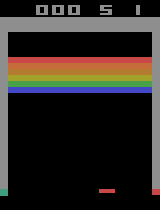
\includegraphics[height=2cm]{./imgs/br0.png}};
		\node [dot, right=0.7cm of frame] (input) {};

		% Encoders
		\matrix [
			right=of input, row sep=1.2cm, column sep=0.5cm, nodes={anchor=center},
		] (encoders) {
			\node [block] (encoder1) {Encoder \\ (region 1)}; \&
			\node [dot] (encoded1) {}; \\
			\node [block] (encoder2) {Encoder \\ (region 2)}; \&
			\node [dot] (encoded2) {}; \\
		};

		% Boolean functions & output
		\matrix [
			right=of encoders, nodes={anchor=center},
			row sep=0.3cm, column sep=1.6cm, label distance=0.4cm,
		] (boolfns) {
			\node [block] (boolfn1) {Boolean fn 1}; \&
			\node [label=right:Fluent 1] (output1) {0}; \\
			\node [block] (boolfn2) {Boolean fn 2}; \&
			\node [label=right:Fluent 2] (output2) {1}; \\
			\node [block] (boolfn3) {Boolean fn 3}; \&
			\node [label=right:Fluent 3] (output3) {0}; \\
		};

		% Output
		\node [
			draw, rectangle, gray, inner sep=0pt, fit=(output1) (output3)
			] (outputs) {};

		% Flow
		\draw (frame) to (input);
		\draw [->] (input) edge (encoder1) edge (encoder2);
		\draw (encoder1) to (encoded1);
		\draw (encoder2) to (encoded2);
		\draw [->] (encoded1) edge (boolfn1.west) edge (boolfn2.west);
		\draw [->] (encoded2) edge (boolfn3.west);
		\draw [->] (boolfn1) to (output1);
		\draw [->] (boolfn2) to (output2);
		\draw [->] (boolfn3) to (output3);

		% Models
		\begin{scope}[
				class label/.style={
					anchor=west, xshift=-1em, yshift=2ex,
					font=\tt\footnotesize, inner sep=0pt, outer sep=3pt,}
			]
			\node [class label] (class features1) at (encoder1.north west)
				{LocalFeatures};
			\node [class label] (class features2) at (encoder2.north west)
				{LocalFeatures};
			\node [class label] (class bools) at (boolfns.north west)
				{BooleanFunctionsArray};
			\node [class label, xshift=-1.2em, yshift=2.5ex]
				(class fluents) at (class features1.north west) {Fluents};
		\end{scope}
		\begin{pgfonlayer}{below}
			\node (encoding1 class box) [
				draw=\encodingColor, fill=\encodingColor!30!white, inner sep=5pt,
					fit=(class features1) (encoder1)] {};
			\node (encoding2 class box) [
				draw=\encodingColor, fill=\encodingColor!30!white, inner sep=5pt,
				fit=(class features2) (encoder2)] {};
			\node (bools class box) [
				draw=\boolsColor, fill=\boolsColor!30!white, inner sep=5pt,
				fit=(class bools) (boolfn3.south east)] {};
		\end{pgfonlayer}
		\begin{pgfonlayer}{beloww}
			\node (fluents class box) [
				draw=\fluentsColor, fill=\fluentsColor!30!white, inner sep=5pt,
				fit={(class fluents) (encoding1 class box) (encoding2 class box)
					(bools class box)}] {};
		\end{pgfonlayer}

		% Annotations
		\coordinate (annotations y) at ($(fluents class box.south)+(0,-0.7)$);
		\begin{pgfonlayer}{below}
			\node (input-annotation) at (input|-annotations y) {Input};
			\node (encoding-annotation) at (encoded1|-annotations y) {Encodings};
			\node (outputs-annotation) at (outputs|-annotations y) {Predictions};
			\draw [pin line] (input) -- (input-annotation);
			\draw [pin line] (encoded1) -- (encoding-annotation);
			\draw [pin line] (outputs) -- (outputs-annotation);
		\end{pgfonlayer}
	\end{tikzpicture}
	\caption{The disposition of the various classes corresponding to the general
	scheme of Figure~\vref{fig:model-scheme}.}
	\label{fig:fluents-classes}
\end{figure}
All the initialization parameters reflect the command line arguments. For
instance, the \verb|--network| command chooses the number of units and layers
of each encoder. Also, \verb|--train| select which of these inner models
should be trained, when we call the object \verb|compute_all| function.
Depending on which model we're working on, both the computation graph and the
metrics saved greatly change.

